\chapter{シミュレーション実験}\label{chap:simulation_experiment}

\section{はじめに}
本章では、3章にて提案したアルゴリズムをMCLに実装し、
シミュレータ環境にて実装したアルゴリズムの評価をする。

\section{シミュレータ環境について}

提案したアルゴリズムを評価するために図\ref{fig:sim_world}のような
シミュレータ環境を用いた。図\ref{fig:sim_world}の環境は図\ref{fig:unknown-obstacles}
の実環境を模したものであり、図\ref{fig:known-obstacles}の2次元マップを
縦方向に伸ばすことによって作成した3次元の環境である。
シミュレータ環境内で使用したロボットは、
Raspberry Pi Cat(以下ラズパイキャット)をモデリングしたものである。

\begin{figure}[h]
  \begin{center}
    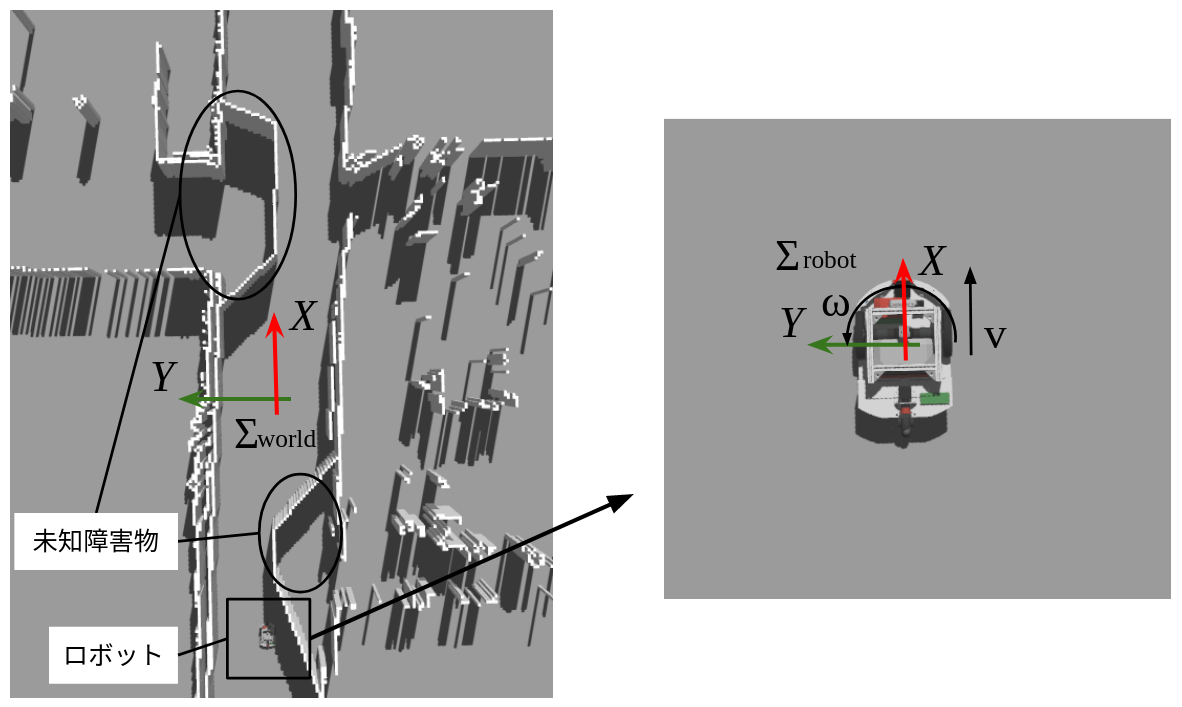
\includegraphics[width=0.98\linewidth]{figs/sim_world.png}
    \caption{使用したシミュレータ環境とロボット}
    \label{fig:sim_world}
  \end{center}
\end{figure}

\newpage

また、図~のようにシミュレータ環境は未知障害物有りと無しとで2通り用意した。
未知障害物は、地図に無い障害物である。

\begin{figure}[htbp]
  \begin{minipage}[b]{0.5\linewidth}
    \centering
    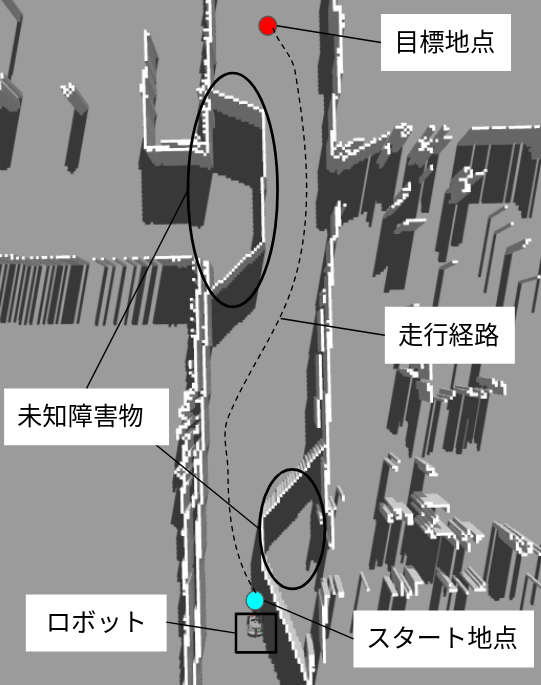
\includegraphics[keepaspectratio, scale=0.32]{figs/gazebo_unknown_obstacles.png}
    \caption{未知障害物有り}
    \label{fig:gazebo_unknown}
  \end{minipage}
  \begin{minipage}[b]{0.5\linewidth}
    \centering
    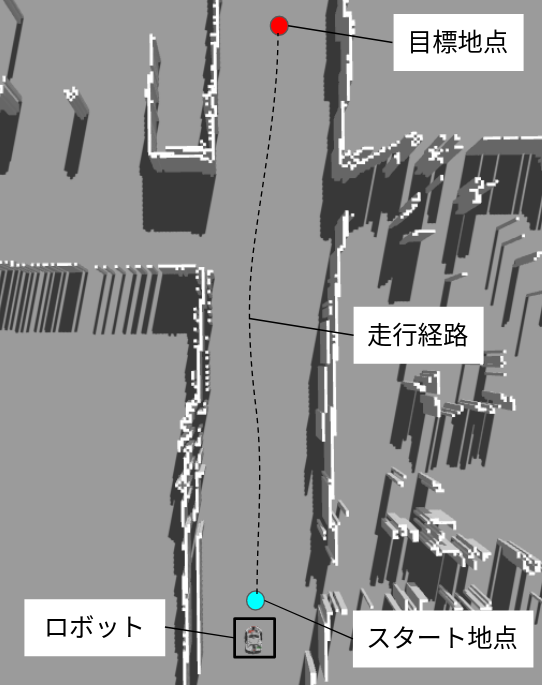
\includegraphics[keepaspectratio, scale=0.32]{figs/gazebo_known_obstacles.png}
    \caption{未知障害物無し}
    \label{fig:gazebo_known}
  \end{minipage}
\end{figure}

\section{ソフトウェアの仕様}

シミュレータ環境およびロボットの制御システムとして、ROSを用いる。

\section{MCLに提案したアルゴリズムの実装}

提案したアルゴリズムを実装する基になるパッケージとして、自己位置推定用
のROSパッケージとして公開されているemclを用いる。
このemclをフォークして、〜というブランチで実装を行った。
実装後のコミット番号は〜であり、このコミット番号において実装した内容について説明していく。

emclでは、基本的なパーティクルフィルタの関数は〜.cppにて実装されているおり、それらの関数を
.cppにて関数の呼び出しを行っている。
まず、.cppに観測パターンを用意するための関数を追加する。
そして、パーティクルの初期化と同時に各パーティクルに
図~のようなランダムな観測パターンを与える。
次に与えられた観測パターンを基に各パーティクルは事前に求められた尤度場により、〜にて尤度計算を行う。
この尤度計算では、未知障害物を含まない良い観測パターンを持ったパーティクルの尤度は高く、
未知障害物を含む良くない観測パターンを持ったパーティクルの尤度は低くなる。
尤度計算後は、パーティクルのばらつきを低減するためにリサンプリングを行う。
リサンプリングでは、ある観測パターンに収束し続けないように、〜にて$N$個のパーティクルのうち$\frac{N}{10}$
のパーティクルをサンプルし、ランダムな観測パターンをそれぞれに与える。
以上の実装により、提案したアルゴリズムを実装したMCLでは尤度計算による観測パターンの評価と
リサンプリングによるランダムな観測パターンの追加によって、未知障害物に対応した観測パターンを求める。

\section{実装したアルゴリズムの評価}

図〜のシミュレータ環境用いて、提案したアルゴリズムを実装したMCLの評価を行う。
評価することは、未知障害物が合った場合の尤度と観測パターンである。
そして、move\_baseによるナビゲーションによって、図\ref{fig:gazebo_unknown}, \ref{fig:gazebo_known}
のようにスタート地点から目標地点までスタックせずに到達できるかも評価を行う。
また、emclにはパーティクルフィルタによる自己位置推定の他に膨張リセットによって
自己位置推定の回復を行う機能が実装されている。
このリセットは、リセットの閾値にパーティクルの尤度を用いており、
未知障害物があった時に不用に働いてしまうことがあるため、
実装したアルゴリズムによって、改善されるのか評価を行う。
4.5.1では、提案したアルゴリズムの実装がない場合、4.5.2では提案したアルゴリズムの実装がある場合
のemclによる自己位置推定について、それぞれ評価をまとめる。

\subsection{提案したアルゴリズムの実装無し}

\subsubsection{未知障害物有りかつ自己位置推定のリセット有り, 無しの場合の走行}

\begin{figure}[htbp]
  \begin{minipage}[b]{0.5\linewidth}
    \centering
    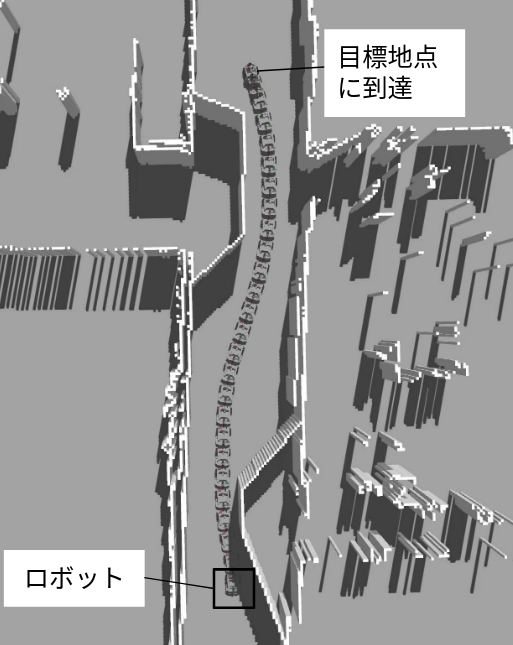
\includegraphics[keepaspectratio, scale=0.32]{figs/no_implementation_no_reset.png}
    \caption{未知障害物有り}
    \label{fig:gazebo_unknown}
  \end{minipage}
  \begin{minipage}[b]{0.5\linewidth}
    \centering
    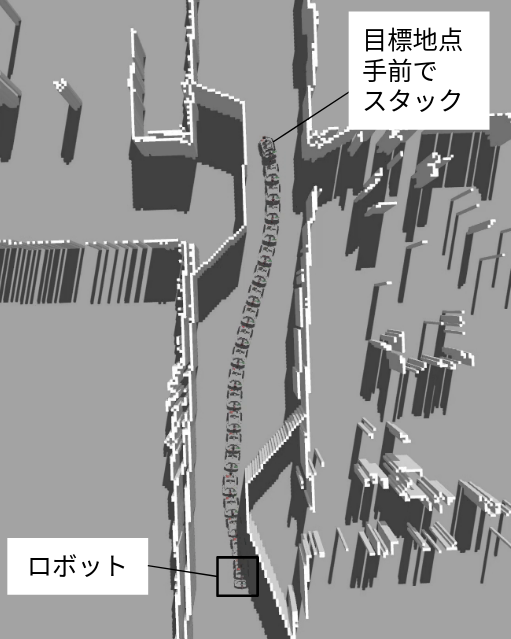
\includegraphics[keepaspectratio, scale=0.32]{figs/no_implementation_with_reset.png}
    \caption{未知障害物無し}
    \label{fig:gazebo_known}
  \end{minipage}
\end{figure}

\subsubsection{未知障害物有り, 無しの場合の尤度}

\subsection{提案したアルゴリズムの実装有り}

\subsubsection{未知障害物有りの場合の走行}

\subsubsection{未知障害物有りかつ自己位置推定のリセット有り, 無しの場合の走行}

\subsubsection{未知障害物有り, 無し場合の尤度と観測パターン}

